%&fduthesis
%TC:ignore
\PassOptionsToPackage{OT1}{fontenc}
\PassOptionsToPackage{amsmath, thmmarks}{ntheorem}
\RequirePackage{
  amsmath,
  ctexhook,
  ctexpatch,
  fancyhdr,
  fix-cm,
  fontenc,
  graphicx,
  hyperref,
  ifvtex,
  l3keys2e,
  ntheorem,
  tikz,
  xcolor,
  xparse,
  xtemplate,
  zhnumber,
}
\let\maketitle\undefined

% tikz
\usetikzlibrary{arrows.meta, decorations.markings}
\tikzset{
  ->-/.style = {
    decoration = {
      markings,
      mark = at position #1 with {\arrow{Stealth}},
    },
    postaction = {decorate},
  },
}

\endofdump
%TC:endignore

\documentclass[type=doctor,oneside]{fduthesis}

\usepackage{enumitem}
\usepackage{tikz}

% fduthesis
\fdusetup{
  style = {
    font = libertinus,
    cjk-font = founder,
    footnote-style = libertinus,
    fullwidth-stop = mapping,
    bib-backend = bibtex,
    bib-resource = {main.bib},
  },
  info = {
    title = {论文标题},
    title* = {Thesis Title},
    author = {曾祥东},
    supervisor = {孔令欣\quad 教授},
    major = {理论物理},
    degree = academic,
    department = {物理学系},
    student-id = {18110190010},
    % date = {2023 年 1 月 1 日},
    keywords = {不确定关系, 量子力学, 理论物理},
    keywords* = {Uncertainty principle, quantum mechanics, theoretical physics},
    clc = {O413.1},
  }
}

% enumitem
\setlist{itemsep=0pt}

% tikz
\usetikzlibrary{arrows.meta, decorations.markings}
\tikzset{
  ->-/.style = {
    decoration = {
      markings,
      mark = at position #1 with {\arrow{Stealth}},
    },
    postaction = {decorate},
  },
}

% Hacks
\ExplSyntaxOn
\__fdu_patch_cmd:Nnn \__fdu_load_cjk_font_founder:
  { \__fdu_setCJKmainfont:n  { FZShuSong-Z01 } }
  { \__fdu_setCJKmainfont:nn { FZShuSong-Z01 } { BoldFont = FZXiaoBiaoSong-B05 } }
\def\hypersetup{\kvsetkeys{Hyp}}
\cs_set:Npn \fdu_allow_url_break:
  {
    \cs_set:Npn \UrlBreaks
      {
        \do \. \do \@ \do \\ \do \/ \do \! \do \_ \do \| \do \; \do \>
        \do \] \do \) \do \, \do \? \do \& \do \' \do  + \do \= \do \#
      }
  }
\ExplSyntaxOff

\AtBeginDocument{
  \setlength{\bibsep}{4pt plus 2pt minus 1pt}
}

% Math commands
\newcommand{\dd}{{\mathrm{d}}}
\newcommand{\ee}{{\mathrm{e}}}
\newcommand{\ii}{{\mathrm{i}}}
\newcommand{\id}{{\mathrm{id}}}
\newcommand{\1}{{\mathbb{1}}}
\newcommand{\bm}[1]{{\symbf{#1}}}
\newcommand{\ldual}[1]{{}^\vee\mspace{-2mu}#1}
\newcommand{\dv}[2]{\frac{\mathrm{d}#1}{\mathrm{d}#2}}
\newcommand{\pdv}[2]{\frac{\partial#1}{\partial#2}}
\NewDocumentCommand{\ket}{sm}{%
  \IfBooleanTF{#1}{|#2\rangle}{\left|#2\right\rangle}}
\DeclareMathOperator{\Hom}{Hom}
\DeclareMathOperator{\End}{End}
\DeclareMathOperator{\tr}{tr}

\newcommand{\tikzinput}[1]{\input{includes/tikz/#1.tex}}

%TC:envir fusionrules [ignore] text
\newenvironment{fusionrules}[1]{%
  \begingroup
    \renewcommand{\arraystretch}{0.8}%
    \begin{tabular}{#1}
      \hline
}{%
      \hline
    \end{tabular}
  \endgroup
}

\begin{document}

\frontmatter

\tableofcontents
\listoffigures

\begin{abstract}
  中文摘要
\end{abstract}

\begin{abstract*}
  English abstract
\end{abstract*}

\mainmatter

\chapter{张量范畴与弦网模型}

\section{范畴论基础}

\emph{范畴论} (category theory) 用以抽象地刻画一些数学结构之间的关系,它主要描述了“对象”之间的作用,即\emph{映射} (mapping)。拓扑序理论中所研究的,正是带有了某些附加结构的范畴。

一个\emph{范畴} $\mathcal{C}$ 由其中的\emph{对象} (object) $x\in\mathcal{C}$ 和这些对象之间的\emph{态射} (morphism) $f\colon x\to y$ 组成。对象之间的态射满足以下三个条件:
\begin{itemize}
  \item \emph{复合性} (composition):对于范畴 $\mathcal{C}$ 中的对象 $x$、$y$、$z$,若 $f\colon x\to y$ 和 $g\colon y\to z$ 为态射,则存在复合态射 $g\circ f\colon x\to z$;
  \item \emph{结合律} (associativity):若 $\mathcal{C}$ 中有态射 $f\colon x\to y$、$g\colon y\to z$、$h\colon z\to w$,则有
    \begin{equation}
      (h\circ g)\circ f = h\circ (g\circ f);
    \end{equation}
  \item \emph{单位元} (identity):对于 $\forall x\in\mathcal{C}$,都存在恒等态射 $\id_x\colon x\to x$,使得
    \begin{equation}
      f \circ \id_x = \id_x \circ f = f, \quad \forall f\colon x\to y.
    \end{equation}
\end{itemize}
态射也可记为 $f\in\Hom_{\mathcal{C}}(x,y)$,其中 $\Hom_{\mathcal{C}}(x,y)$ 称为同态集 (hom-set)。如果 $x=y$,则称 $f$ 为\emph{自同态} (endomorphism),记为 $f\in\End_{\mathcal{C}}(x)$。

\emph{函子} (functor) 是范畴之间保结构的映射。具体而言,对于范畴 $\mathcal{C}$、$\mathcal{D}$,函子 $F\colon\mathcal{C}\to\mathcal{D}$ 会将 $\mathcal{C}$ 中的对象 $x$ 映射到 $\mathcal{D}$ 中的对象 $F(x)$,而将 $\mathcal{C}$ 中的态射 $f\colon x\to y$ 映射到 $\mathcal{D}$ 中的态射 $F_f\colon F(x)\to F(y)$,并且保持复合性与单位元的成立,即
\begin{align}
  F_{\id_x} &= \id_{F(x)} \colon F(x) \to F(x), \quad \forall x\in\mathcal{C}, \\
  F_{g\circ f} &= F_g \circ F_f \colon F(x) \to F(z), \quad \forall f\colon x\to y, \, g\colon y\to z.
\end{align}

在函子之上可进一步定义\emph{自然变换} (natural transformation)。对于两个函子 $F\colon\mathcal{C}\to\mathcal{D}$ 和 $G\colon\mathcal{C}\to\mathcal{D}$,自然变换 $\tau\colon F\Rightarrow G$ 由其分量 $\tau_x$(这是范畴 $\mathcal{D}$ 中的一个态射)定义:
\begin{equation}
  \tau_x\colon F(x)\to G(x), \quad \forall x\in\mathcal{C},
\end{equation}
它满足
\begin{equation}
  \tau_y \circ F_f = G_f \circ \tau_x, \quad \forall f\colon x\to y.
\end{equation}
如图~\ref{fig:natural-transformation},自然变换可以用交换图来直观地表示。若 $\tau$ 的每一分量 $\tau_x$ 均可逆(即存在 $\tau_x^{-1}$ 使得 $\tau^{-1}_x\circ\tau_x=\id_{F(x)}$ 且 $\tau_x\circ\tau^{-1}_x = \id_{G(x)}$),则称其为\emph{自然同构} (natural isomorphism),我们用 $\similarrightarrow$ 来表示。

\begin{figure}[htb]
  \centering
  \begin{tabular}{c@{\qquad}c}
    \includegraphics{images/natural-transformation-1.pdf} &
    \includegraphics{images/natural-transformation-2.pdf} \\
    (a) & (b)
  \end{tabular}
  \caption[自然变换对应的交换图]{自然变换对应的交换图。(a) 此图是“可交换的”,即从 $F(x)$ 到 $G(y)$ 的两条路径等价;(b) 对于结合律的“提升”,图中三棱柱的三个侧面都是可交换的。}
  \label{fig:natural-transformation}
\end{figure}

\begin{example}
  对于任意的交换环 $K$,以其中元素构成的 $n\times n$ 的非奇异矩阵组成了一般线性群 $GL_n(K)$。对于环同态 $f\colon K\to L$,显然可以构建群同态 $GL_n f\colon GL_n(K)\to GL_n(L)$。因此,$GL_n$ 即为交换环范畴 $\mathbf{CRng}$ 到群范畴 $\mathbf{Grp}$ 的函子。

  设非奇异矩阵 $M\in GL_n(K)$,则其行列式 $\det_K(M)$ 为 $K$ 中的可逆元(即单位),因而 $\det_K$ 是群同态 $GL_n(K)\to K^\times$,其中 $K^\times$ 为 $K$ 的可逆元群。另一方面,当把环同态 $f$ 限制在可逆元群上时,可得群同态 $f^\times\colon K^\times\to L^\times$,因而 $(\cdot)^\times$ 同样也是 $\mathbf{CRng}$ 到 $\mathbf{Grp}$ 的函子。根据定义,$\det\colon GL_n\Rightarrow(\cdot)^\times$ 即为自然变换,它满足 $\det_L\circ\,GL_n f=f^\times\circ \det_K$。
\end{example}

% \begin{example}
%   在 Haskell 编程语言中,类型为范畴 $\mathbf{Hask}$ 中的对象,而纯函数为态射。函子可由类型类 (type class) 来定义,例如 \verb|List| 可以将类型 \verb|T| 构造为对应的数组 \verb|[T]|,并且通过 \verb|fmap| 将以 \verb|T| 类型为参数的纯函数转换为以 \verb|[T]| 类型为参数的纯函数。自然变换则由参数多态 (parametric polymorphism) 实现。例如,一个安全的(不引发异常)返回数组首元素的函数可按下面的方式定义:
% \begin{verbatim}
%   head :: [T] -> Maybe T
%   head []     = Nothing
%   head (x:xs) = Just x
% \end{verbatim}
%   因此 \verb|head| 函数是从 \verb|List| 到 \verb|Maybe| 的自然变换。
% \end{example}

\emph{弦图} (string diagram) 可以更直观地描述范畴的概念。其中,带箭头的直线或曲线代表对象,盒子代表态射:
\begin{equation}
  f\colon x\to y \quad \coloneq \quad
  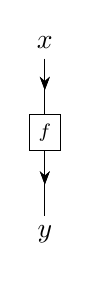
\begin{tikzpicture}[baseline=1cm]
  \draw [->-=0.2, ->-=0.8]
    (0,2) node [above] {$x$} -- (0,0) node [below] {$y$}
    (0,1) node [draw, fill=white, anchor=base] {$\scriptstyle f$};
\end{tikzpicture}
 \, .
\end{equation}
这样态射的复合就可以表示为连在一起的两个盒子:
\begin{equation}
  \begin{tikzpicture}[baseline=1.9em, thick]
  \draw [->-=0.2, ->-=0.86]
    (0,4) node [above] {$x$} -- (0,0) node [below] {$z$}
    (0,2) node [morphism box, minimum size=1.5em] {$g\circ f$};
  \draw (2,2) node [anchor=base] {=};
  \draw [->-=0.53]
    (4,5)   node [above] {$x$} -- (4,-1) node [below] {$z$}
    (4.8,2) node {$y$}
    (4,3.5) node [morphism box, minimum size=1.5em] {$f$}
    (4,0.5) node [morphism box, minimum size=1.5em] {$g$};
\end{tikzpicture}
.
\end{equation}

\section{张量范畴与融合范畴}

\subsection{张量范畴}

我们可以在范畴中引入一些结构,使其具有新的特性。引入了张量积的范畴为\emph{张量范畴} (tensor category)。它最基本也最重要的例子是向量空间(或对应的范畴 $\mathbf{Vec}$),其中的张量积结构即为两个向量空间和相应线性变换的直积。一个张量范畴 $\mathcal{C}$ 由下面的条件定义:
\begin{itemize}
  \item \emph{张量积} (tensor product) $\otimes\colon\mathcal{C}\times\mathcal{C}\to\mathcal{C}$ 和\emph{单位对象} (unit object) $\1\in\mathcal{C}$;
  \item \emph{结合子} (associator) $\alpha$,它是一个自然同构:
    \begin{equation}
      \alpha_{x,y,z} \colon (x\otimes y)\otimes z \similarrightarrow x\otimes(y\otimes z), \quad \forall x,y,z \in \mathcal{C};
    \end{equation}
  \item \emph{左右单位子} (left/right unitor),同样也是自然同构:
    \begin{equation}
      \lambda_x \colon \1\otimes x \similarrightarrow x, \quad
      \rho_x    \colon x\otimes\1  \similarrightarrow x, \quad
      \forall x \in \mathcal{C}.
    \end{equation}
\end{itemize}
它们需要满足五边形方程和三角形方程(图~\ref{fig:pentagon-triangle-equation})。

\begin{figure}[htb]
  \centering
  \begin{tabular}{cc}
    \includegraphics{images/pentagon-equation.pdf} &
    \includegraphics{images/triangle-equation.pdf} \\
    (a) & (b)
  \end{tabular}
  \caption[五边形方程和三角形方程对应的交换图]{五边形方程 (a) 和三角形方程 (b) 对应的交换图。}
  \label{fig:pentagon-triangle-equation}
\end{figure}

如果上述定义中的 $\similarrightarrow$ 可以取为等号,则称该张量范畴是\emph{严格} (strict) 的,此时 $\alpha$、$\lambda$ 和 $\rho$ 均为恒等变换。根据 MacLane \emph{一致性定理} (coherence theorem),每个张量范畴都等价于一个严格张量范畴。因此我们之后可以只考虑严格张量范畴的情况。此时张量积表达式中的括号和单位对象都可以忽略。

一个张量范畴也是一个\emph{幺半群} (monoid),因为范畴的单位对象可以作为群的单位元,而张量积可以作为群乘法。所以张量范畴也被称为\emph{幺半范畴} (monoidal category)。

\subsection{对偶}

类似于对偶空间的概念,我们可以在张量范畴中引入\emph{对偶} (dual) 的概念。$x\in\mathcal{C}$ 的\emph{右对偶} (right dual) $x^\vee$ 通过以下两个态射定义:
\begin{equation}
  e_x\colon x^\vee\otimes x\to\1, \quad i_x\colon\1\to x\otimes x^\vee,
\end{equation}
它们需要满足\emph{刚性公理} (rigidity axioms):
\begin{equation}
  \begin{aligned}
    (\id_x\otimes e_x) \circ (i_x\otimes\id_x) &= \id_x, \\
    (e_x\otimes\id_{x^\vee}) \circ (\id_{x^\vee}\otimes i_x) &= \id_{x^\vee}.
  \end{aligned}
\end{equation}
如果在弦图中省略单位元(对应于物理中的真空态),则 $e_x$ 和 $i_x$ 可以表示为
\begin{equation}
  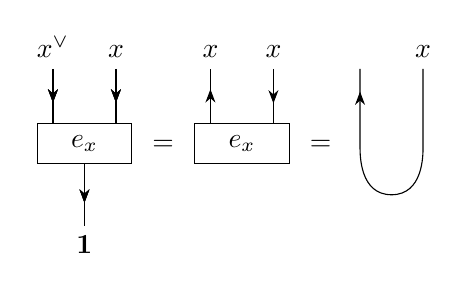
\begin{tikzpicture}[baseline=1cm]
  \draw [->-={1/7}, ->-={10/21}, ->-=0.9]
    (0  ,2) node [above=4pt, anchor=base] {$x^\vee$} -- ++ (0,-1)
    (0.8,2) node [above=4pt, anchor=base] {$x$}      -- ++ (0,-1)
    (0.4,1) -- ++ (0,-1) node [below] {$\mathbf{1}$};
  \draw (0.4,1) node [draw, minimum width=1.2cm, minimum height=0.5cm, fill=white, anchor=base] {$e_x$};
  \draw (1.4,1.03) node {=};
  \draw [->-=0.74] (2,1) -- ++ (0,1) node [above=4pt, anchor=base] {$x$};
  \draw [->-=0.44] (2.8,2) node [above=4pt, anchor=base] {$x$} -- ++ (0,-1);
  \draw (2.4,1) node [draw, minimum width=1.2cm, minimum height=0.5cm, fill=white, anchor=base] {$e_x$};
  \draw (3.4,1.03) node {=};
  \draw [->-=0.92] (4.7,2) node [above=4pt, anchor=base] {$x$}
    -- (4.7,1) .. controls (4.7,0.9) and (4.7,0.4) .. (4.3,0.4)
               .. controls (3.9,0.4) and (3.9,0.9) .. (3.9,1  ) -- (3.9,2);
\end{tikzpicture}
,
  \qquad
  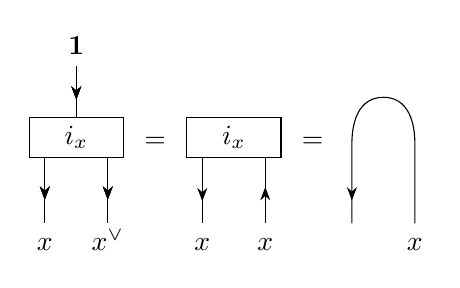
\begin{tikzpicture}[baseline=1cm]
  \draw [->-={1/7}, ->-=0.567, ->-=0.9]
    (0.4,2) node [above=4pt, anchor=base] {$\mathbf{1}$} -- ++ (0,-1)
    (0  ,1) -- ++ (0,-1) node [below=10pt, anchor=base] {$x$}
    (0.8,1) -- ++ (0,-1) node [below=10pt, anchor=base] {$x^\vee$};
  \draw (0.4,1) node [draw, minimum width=1.2cm, minimum height=0.5cm, fill=white, anchor=base] {$i_x$};
  \draw (1.4,1.03) node {=};
  \draw [->-=0.72] (2  ,1) -- ++ (0,-1) node [below=10pt, anchor=base] {$x$};
  \draw [->-=0.46] (2.8,0) node [below=10pt, anchor=base] {$x$} -- ++ (0,1);
  \draw (2.4,1) node [draw, minimum width=1.2cm, minimum height=0.5cm, fill=white, anchor=base] {$i_x$};
  \draw (3.4,1.03) node {=};
  \draw [->-=0.92] (4.7,0) node [below=10pt, anchor=base] {$x$}
    -- (4.7,1) .. controls (4.7,1.1) and (4.7,1.6) .. (4.3,1.6)
               .. controls (3.9,1.6) and (3.9,1.1) .. (3.9,1  ) -- (3.9,0);
\end{tikzpicture}
.
\end{equation}
这可以类比于量子力学中的湮灭与产生算符。(右对偶的)刚性公理则可表示为
\begin{equation}
  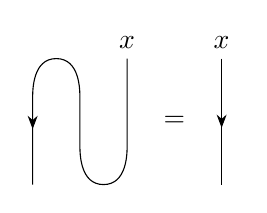
\begin{tikzpicture}[baseline=0.8cm]
  \draw [->-=0.87] (1.2,1.6) node [above] {$x$}
    -- (1.2,0.5)
    .. controls (1.2,0.4) and (1.2,0.0) .. (0.9,0.0)
    .. controls (0.6,0.0) and (0.6,0.4) .. (0.6,0.5)
    -- (0.6,1.1)
    .. controls (0.6,1.2) and (0.6,1.6) .. (0.3,1.6)
    .. controls (0.0,1.6) and (0.0,1.2) .. (0.0,1.1)
    -- (0.0,0.0);
  \draw (1.8,0.8) node {=};
  \draw [->-=0.55] (2.4,1.6) node [above] {$x$} -- (2.4,0);
\end{tikzpicture}
,
  \qquad
  \input{includes/tikz/rigidity-axioms-2.tex}.
  \label{eq:rigidity-axioms-diagrams}
\end{equation}

同理,我们还可以定义\emph{左对偶} (left dual):
\begin{equation}
  e'_x \colon x\otimes \ldual{x}\to\1, \quad i'_x\colon \1\to\ldual{x}\otimes x.
  \label{eq:left-dual}
\end{equation}
这实际上只需要对上面的图沿水平方向做一下镜像操作。如果 $\mathcal{C}$ 中的每个对象既有左对偶也有右对偶,则称其为是\emph{刚性} (rigid) 的或\emph{自治} (autonomous) 的;而如果 $\forall x\in\mathcal{C}$,都有 $x=x^\vee$,则称 $\mathcal{C}$ 是\emph{自对偶} (self-dual) 的。

\subsection{中枢与球状结构}

我们知道有限维向量空间 $V$ 的二重对偶 $V^{\vee\vee}$ 同构于 $V$。这在张量范畴中的推广即为\emph{中枢} (pivotal) 结构,它是由以下的自然同构给出的:
\begin{equation}
  \delta_x \colon x \similarrightarrow x^{\vee\vee}, \quad \forall x\in\mathcal{C},
\end{equation}
且需满足
\begin{equation}
  \delta_{x\otimes y} = \delta_x\otimes\delta_y, \quad
  \delta_\1 = \id_\1, \quad
  \delta_{x^\vee} = (\delta_x^\vee)^{-1}.
\end{equation}
根据右对偶的定义,可有
\begin{equation}
  e_x\colon x^\vee\otimes x \similarrightarrow x^\vee\otimes x^{\vee\vee}\to\1, \quad
  i_x\colon \1\to x\otimes x^\vee \similarrightarrow x^{\vee\vee}\otimes x^\vee.
\end{equation}
对比式~\eqref{eq:left-dual},可以发现 $x^{\vee\vee}$ 也是 $x^\vee$ 的左对偶。若令 $y=x^\vee$,即有 $\ldual{y}=y^\vee$,也就是说在中枢范畴中可以不再区分左右对偶。

对于中枢范畴 $\mathcal{C}$ 中的自同态 $f\in\End_{\mathcal{C}}(x)$,可以定义\emph{左右迹} (left/right trace):
\begin{equation}
  \begin{aligned}
    \tr_{\text{L}} f &\colon \1 \xrightarrow{i_{x^\vee}} x^\vee\otimes x^{\vee\vee}
                                \xrightarrow{\id_{x^\vee}\otimes\delta_x^{-1}} x^\vee\otimes x
                                \xrightarrow{\id_{x^\vee}\otimes f} x^\vee\otimes x
                                \xrightarrow{e_x} \1, \\
    \tr_{\text{R}} f &\colon \1 \xrightarrow{i_x} x\otimes x^\vee
                                \xrightarrow{f\otimes\id_{x^\vee}} x\otimes x^\vee
                                \xrightarrow{\delta_x\otimes\id_{x^\vee}} x^{\vee\vee}\otimes x^\vee
                                \xrightarrow{e_{x^\vee}} \1.
  \end{aligned}
\end{equation}
当 $f=\id_x$ 时,还可以定义\emph{左右维数} (left/right dimension):
\begin{equation}
  \dim_{\text{L}} x \coloneq \tr_{\text{L}}\id_x, \quad
  \dim_{\text{R}} x \coloneq \tr_{\text{R}}\id_x.
  \label{eq:left-right-dimension}
\end{equation}
迹和维数可以用下图来描述:
\begin{equation}
  \tr_{\text{L}}  f = \begin{tikzpicture}[thick, baseline=-0.2em]
  \draw (-2,-1) node [left] {$b$} -- (1,0.5)
    .. controls (1.4, 0.7) and (1.7, 0.8) .. (1.9, 0.8)
    .. controls (2.2, 0.8) and (2.5, 0.5) .. (2.5, 0.0) node [right] {$i$}
    .. controls (2.5,-0.5) and (2.2,-0.8) .. (1.9,-0.8)
    .. controls (1.7,-0.8) and (1.4,-0.7) .. (1.0,-0.5)
    -- (-2,1) node [left] {$a$}
       (7.0,-0.5)
    .. controls (6.1,-0.3) and (5.5,-0.1) .. (5.5, 0.3)
    .. controls (5.5, 0.7) and (6.1, 0.9) .. (7.0, 0.9)
    .. controls (7.9, 0.9) and (8.5, 0.7) .. (8.5, 0.3) node [right] {$i$}
    .. controls (8.5,-0.1) and (7.9,-0.3) .. (7.0,-0.5);
  \draw [fill=MaterialRed]   (0,0)    circle [radius=0.6];
  \draw [fill=MaterialGreen] (7,-0.4) circle [radius=0.6];
  \draw [node font=\normalsize]
    (0,-2.5) node {$A_{abii}$}
    (7,-2.5) node {$B_{ii}$};
\end{tikzpicture}
 \, , \quad
  \tr_{\text{R}}  f = 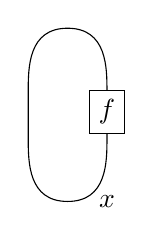
\begin{tikzpicture}[baseline=1.05cm]
  \draw [->-=0.27]
      (0.5,0.0)
    .. controls (1.0,0.0) and (1.0,0.5) .. (1.0,0.8)
    -- (1.0,1.4)
    .. controls (1.0,1.7) and (1.0,2.2) .. (0.5,2.2)
    .. controls (0.0,2.2) and (0.0,1.7) .. (0.0,1.4)
    -- (0.0,0.8)
    .. controls (0.0,0.5) and (0.0,0.0) .. cycle
    (1.0,0.0) node {$x$}
    (1.0,1.05) node [draw, fill=white, anchor=base] {$f$};
\end{tikzpicture}
 \, ; \quad
  \dim_{\text{L}} x = 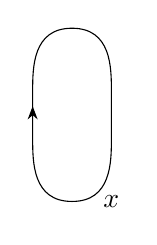
\begin{tikzpicture}[baseline=1.05cm]
  \draw [->-=0.27]
      (0.5,0.0)
    .. controls (0.0,0.0) and (0.0,0.5) .. (0.0,0.8)
    -- (0.0,1.4)
    .. controls (0.0,1.7) and (0.0,2.2) .. (0.5,2.2)
    .. controls (1.0,2.2) and (1.0,1.7) .. (1.0,1.4)
    -- (1.0,0.8)
    .. controls (1.0,0.5) and (1.0,0.0) .. cycle
    (1.0,0.0) node {$x$};
\end{tikzpicture}
 \!, \quad
  \dim_{\text{R}} x = \input{includes/tikz/dimension-2.tex} \!.
\end{equation}
如果对于任意的 $f\in\End_{\mathcal{C}}(x)$ 都有 $\tr_{\text{L}}f=\tr_{\text{R}}f$,则称 $\mathcal{C}$ 是\emph{球状} (spherical) 的。

\subsection{融合范畴}

范畴中还可以引入\emph{直和} (direct sum) 的结构。若范畴 $\mathcal{C}$ 中的对象均可分解为\emph{简单对象} (simple object) 的直和:
\begin{equation}
  x = \bigoplus_{i\in I} n_i x_i, \quad \forall x \in \mathcal{C},
\end{equation}
其中 $x_i\in\mathcal{C}$ 是简单对象,$I$ 是非零简单对象的指标集,而系数 $n_i\in\mathbb{Z}_+$,则称 $\mathcal{C}$ 是一个\emph{半单范畴} (semi-simple category)。简单对象的例子包括向量空间范畴 $\mathbf{Vec}$ 中的一维空间(直线),以及 Abel 群范畴 $\mathbf{Ab}$ 中的单群。

若张量范畴 $\mathcal{C}$ 同时也是半单的,并且简单对象只有有限多个,那么这样的 $\mathcal{C}$ 称为\emph{融合范畴} (fusion category)。此时简单对象的张量积可以写成:
\begin{equation}
  x_a \otimes x_b = \bigoplus_c N_{ab}^c x_c,
\end{equation}
其中 $N_{ab}^c\in\mathbb{Z}_+$,称为\emph{融合系数} (fusion coefficient)。在物理学中一般可以假设 $N_{ab}^c$ 只能取到 0 或 1,即是否允许该融合发生。所有允许的融合称为 \emph{融合规则} (fusion rule)。融合范畴还要与张量范畴的结构相容,这意味着
\begin{equation}
  N_{\1 a}^b = N_{a\1}^b = \delta_{ab}, \quad
  \sum_x N_{ax}^z N_{bc}^x = \sum_y N_{ab}^y N_{yc}^z.
\end{equation}
我们还要求融合范畴是刚性且自对偶的,此时可以证明
\begin{equation}
  N_{ab}^c = N_{ba}^c = N_{ac}^b = N_{ca}^b = N_{bc}^a = N_{cb}^a,
\end{equation}
即融合系数关于所有指标均对称。

定义矩阵 $(N_a)_{bc}\coloneq N_{ab}^c$,根据 Perron--Frobenius 定理,可知 $N_a$ 存在最大的非负特征值,这定义为简单对象 $a$ 的\emph{量子维数} (quantum dimension)或 Perron--Frobenius 维数 $d_a$。可以证明,量子维数与式~\eqref{eq:left-right-dimension} 中通过迹定义的维数是相同的。

融合的逆运算是\emph{拆分} (splitting)。简单对象的融合与拆分都可以用弦图来表示:
\begin{equation}
  \begin{tikzpicture}[baseline=0cm]
  \draw
    (0:0) -- (150:0.5) node [above] {$a$}
    (0:0) -- (30:0.5)  node [above] {$b$}
    (0:0) -- (-90:0.4) node [below] {$c$};
\end{tikzpicture}

  \in \Hom_{\mathcal{C}}(a\otimes b, c) \eqcolon V^{ab}_c, \quad
  \begin{tikzpicture}[baseline=0cm]
  \draw
    (0:0) -- (90:0.4)   node [above] {$c$}
    (0:0) -- (-150:0.5) node [below=0.4cm, anchor=base] {$a$}
    (0:0) -- (-30:0.5)  node [below=0.4cm, anchor=base] {$b$};
\end{tikzpicture}

  \in \Hom_{\mathcal{C}}(c, a\otimes b) \eqcolon V_{ab}^c.
\end{equation}
由于 $\mathcal{C}$ 的刚性和自对偶性,我们可以省略弦图中的箭头。此时,$\Hom_{\mathcal{C}}(a\otimes b,c)$ 和 $\Hom_{\mathcal{C}}(c,a\otimes b)$ 都是向量空间,分别记为 $V^{ab}_c$ 和 $V_{ab}^c$,上面的“融合树”正是对应的基向量。这两个向量空间的维数相等,都等于融合系数 $N_{ab}^c$。

下面我们考虑向量空间 $V^{abc}_d$,它表示从 $a\otimes b\otimes c$ 到 $d$ 的融合。由于 $\mathcal{C}$ 是严格的,$(a\otimes b)\otimes c$ 和 $a\otimes(b\otimes c)$ 的结果相同(都等于 $d$),但却会给出两种融合树的分支结构:
\begin{equation}
  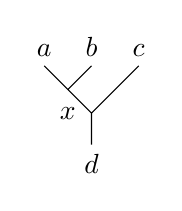
\begin{tikzpicture}[baseline=0]
  \draw
    (0,0)      -- (-0.6,0.6) node [above] {$a$}
    (-0.3,0.3) -- (0,0.6)    node [above] {$b$}
    (0,0)      -- (0.6,0.6)  node [above] {$c$}
    (0,0)      -- (0,-0.4)   node [below] {$d$}
    (-0.3,0) node {$x$};
\end{tikzpicture}

  \in \bigoplus_x V^{ab}_x \otimes V^{xc}_d \simeq V^{abc}_d, \quad
  \input{includes/tikz/f-symbol-2.tex}
  \in \bigoplus_x V^{ay}_d \otimes V^{bc}_y \simeq V^{abc}_d.
\end{equation}
联系这两组基的变换称为 \emph{$F$ 移动} ($F$-move):
\begin{equation}
  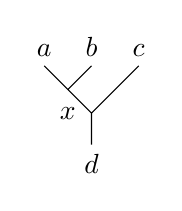
\begin{tikzpicture}[baseline=0]
  \draw
    (0,0)      -- (-0.6,0.6) node [above] {$a$}
    (-0.3,0.3) -- (0,0.6)    node [above] {$b$}
    (0,0)      -- (0.6,0.6)  node [above] {$c$}
    (0,0)      -- (0,-0.4)   node [below] {$d$}
    (-0.3,0) node {$x$};
\end{tikzpicture}

  = \sum_y \, \bigl[ F^{abc}_d \bigr]_{xy}
  \input{includes/tikz/f-symbol-2.tex}.
  \label{eq:f-move}
\end{equation}
式中的系数 $[F^{abc}_d]_{xy}$ 称为 \emph{$F$ 符号} ($F$-symbol),它一共有 6 个指标。$\mathcal{C}$ 中的 $F$ 符号并不是独立的。如图~\ref{fig:f-symbols-pentagon-equation} 所示,它们所满足的约束条件同样也是五边形方程。

\begin{figure}[htb]
  \centering
  \includegraphics{images/f-symbols-pentagon-equation.pdf}
  \caption[$F$ 符号所满足的五边形方程]{$F$ 符号所满足的五边形方程,对应的融合空间是 $\Hom_{\mathcal{C}}(a\otimes b\otimes c\otimes d,e)$,即 $V^{abcd}_e$。}
  \label{fig:f-symbols-pentagon-equation}
\end{figure}

一个融合范畴可由以下几组数据完全确定:
\begin{itemize}
  \item 简单对象的集合 $\{a,b,c,\ldots\}$;
  \item 融合系数 $N_{ab}^c$ 或者对应的融合规则;
  \item $F$ 符号 $[F^{abc}_d]_{xy}$。
\end{itemize}
利用这些数据可以对任意弦图进行化简或求值。如果一个弦图没有端点(即“外腿”),那么它的化简结果将是一个复数。根据上文,我们可以进行的操作有:
\begin{itemize}
  \item 任意的连续变形,这是由刚性公理式~\eqref{eq:rigidity-axioms-diagrams} 和自对偶性保证的;
  \item $F$ 移动,即式~\eqref{eq:f-move};
  \item 环路消除,这会得到相应的量子维数:
    \begin{equation}
      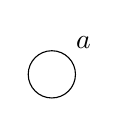
\begin{tikzpicture}[baseline=-0.1cm]
  \draw circle [radius=0.3] (0,0)
    (0.4,0.4) node {$a$};
\end{tikzpicture}

      \! = d_a, \quad
      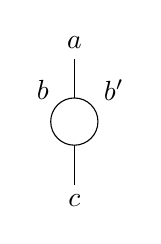
\begin{tikzpicture}[baseline=-0.1cm]
  \draw (0,0.8) node [above] {$a$} -- (0,-0.8) node [below] {$c$};
  \draw [fill=white] circle [radius=0.3] (0,0)
    (-0.4,0.4) node {$b$}
    ( 0.5,0.4) node {$b'$};
\end{tikzpicture}

      \! = \delta_{ac} \sqrt{\frac{d_b d_{b'}}{d_a}} \enspace
      \begin{tikzpicture}[baseline=-0.1cm]
  \draw (0,0.8) -- (0,-0.8)
    (0.3,0.7) node {$a$};
\end{tikzpicture}
.
    \end{equation}
\end{itemize}

\section{拓扑序}

\section{弦网模型}

\chapter{张量网络方法介绍}
\label{chap:tensor-network}

\section{基本概念}

\emph{张量网络} (tensor network)\cite{orus2014practical,bridgeman2017hand,biamonte2017tensor,orus2019tensor,ran2020tensor,evenbly2022practical} 为凝聚态物理、量子信息、机器学习等领域提供了一套统一的描述框架。顾名思义,张量网络就是根据一定规则连接起来张量单元。这里的\emph{张量} (tensor) 可以简单理解为多维数组,即标量(0 维张量)、向量(1 维张量)、矩阵(2 维张量)的推广。

如图~\ref{fig:tensors} 所示,张量网络常利用图形方式来描述,其中圆圈(也可用其他图形)表示张量,延伸出来的腿表示张量的指标。

\begin{figure}[htb]
  \centering
  \includegraphics[width=0.6\textwidth]{images/temp/tensors.pdf}
  \caption[张量单元]{三种张量单元,分别为向量、矩阵和三阶张量。}
  \label{fig:tensors}
\end{figure}

\subsection{基本张量运算}

常用的张量运算包括张量积、缩并、变形等。

\emph{张量积} (tensor product) 其实就是把若干个张量并排放置,并保持指标不变:
\begin{equation}
  (A \otimes B)_{i_1,\dots,i_r,j_1,\dots,j_s} \coloneq A_{i_1,\dots,i_r} B_{j_1,\dots,j_s}.
\end{equation}
图形描述为
\begin{equation}
  [[TODO:]]
\end{equation}

张量的\emph{缩并} (contraction) 是向量内积、矩阵乘法的推广,即对两个张量的某些指标进行求和,得到一个新的张量:
\begin{equation}
  C_{abc} = \sum_k A_{abk} B_{kc} \eqcolon A_{abk} B_{kc}
\end{equation}
这里根据 Einstein 求和约定省略了求和号。张量缩并的图形描述为
\begin{equation}
  \mbox{\includegraphics[width=0.75\textwidth]{images/temp/contraction.pdf}}
\end{equation}
即把需要缩并的腿(指标)连接起来。

同一个张量的指标也可以缩并,这样就得到了\emph{迹} (trace) 或\emph{偏迹} (partial trace):
\begin{equation}
    (\tr_{x,y} A)_{i_1,\dots,i_{x-1},i_{x+1},\dots,i_{y-1},u_{y+1},\dots,i_r}
  = A_{i_1,\dots,i_{x-1},k,i_{x+1},\dots,i_{y-1},k,i_{y+1},\dots,i_r}.
\end{equation}
其图形描述与缩并类似:
\begin{equation}
  [[TODO:]]
\end{equation}
利用图形语言很容易验证 $\tr(AB)=\tr(BA)$:
\begin{equation}
  [[TODO:]]
\end{equation}

张量的\emph{变形} (reshape) 相当于指标的重新组合,例如
\begin{equation}
  \mbox{\includegraphics[width=0.5\textwidth]{images/temp/reshape.pdf}}
\end{equation}
在数值计算中,把一般形状的张量变形为矩阵,往往可以利用为矩阵优化的算法来加速计算。

\subsection{张量分解}

张量的\emph{分解} (decomposition) 可以理解为缩并的逆运算,最常用的是\emph{奇异值分解} (singular value decomposition, SVD),即
\begin{equation}
  M_{ij} = \sum_{k=1}^{\min(m,n)} U_{ik} \Lambda_{kk} V_{kj} = \sum_k U_{ik} \Lambda_{kk} \bigl( V^\dagger \bigr)_{jk},
\end{equation}
其中 $M$ 为 $m\times n$ 矩阵,$\Lambda$ 为对角矩阵(如果行数、列数不等,则相应补零),$U$ 和 $V$ 为幺正矩阵,$V^\dagger$ 表示共轭转置。利用张量的变形,可以很容易地将 SVD 推广为一般形状的张量,用图形描述为
\begin{equation}
  [[TODO:]]
\end{equation}

奇异值分解可以用来获得张量的近似表示。将奇异值($\Lambda$ 矩阵的对角元)按大小排列后,只保留前 $r$ 个值,就得到了秩为 $r$ 的近似张量:
\begin{equation}
  M_{ij} \approx \sum_{k=1}^r U_{ik} \Lambda_{kk} V_{kj}, \quad r < \min(m,n).
\end{equation}
并且可以证明,这种近似表示是所有秩为 $r$ 的张量中最优的。

对于一个一般的张量,原则上我们总可以把它改写为若干个小张量的缩并形式,并保证自由度数目不变。这种改写并不能降低计算复杂度,但我们可以利用奇异值分解把这些小张量替换为对应的近似表示,这样就可以大幅减少总自由度的数目。

在量子力学的语境中,奇异值分解也可表述为 \emph{Schmidt 分解} (Schmidt decomposition):对于 Hilbert 空间 $\mathcal{H}^{\text{L}}\otimes\mathcal{H}^{\text{R}}$,其中的任意量子态 $\ket{\Psi}$ 均可被分解为
\begin{equation}
  \ket{\Psi} = \sum_\alpha \lambda_\alpha \ket{\Phi^{\text{L}}_\alpha} \otimes \ket{\Phi^{\text{R}}_\alpha},
  \label{eq:schmidt-decomposition}
\end{equation}
其中 $\lambda_\alpha$ 称为 \emph{Schmidt 系数} (Schmidt coefficients),而 $\ket{\Phi^{\text{L}}_\alpha}$、$\ket{\Phi^{\text{R}}_\alpha}$ 分别是 $\mathcal{H}^{\text{L}}$、$\mathcal{H}^{\text{R}}$ 中的单位正交基,称为 \emph{Schmidt 向量} (Schmidt vectors)。可以发现 Schmidt 系数和奇异值是等价的,而 Schmidt 向量和幺正矩阵 $U$、$V$ 也是等价的。

\section{矩阵乘积态算法}

接下来介绍几种具体的张量网络及其算法。本文中,我们把这些算法分为两类:一类算法以矩阵乘积态为代表,主要用来处理一维量子多体系统;另一类算法则以张量重整化群为代表,顾名思义,主要用在二维网络的重整化(粗粒近似)操作中。

\subsection{波函数的构造}
\label{subsec:mps-construction}

% \citet{cirac2021matrix}

如图~\ref{fig:mps} 所示,\emph{矩阵乘积态} (matrix product state, MPS)\cite{perez2007matrix,verstraete2008matrix,orus2014practical} 由一系列张量单元首尾相连而成,每个张量单元包含三个指标,没有缩并的称为\emph{物理指标} (physical index),另外两个则称为\emph{虚拟指标} (virtual index) 或\emph{辅助指标} (auxiliary index)。根据具体问题的需要,MPS 可取开放或周期性边界条件。当所研究的系统具有平移对称性时,可以将所有张量单元取为相同值,此时有
\begin{equation}
  % TODO: 周期性边界条件
  \Psi_{i_1 i_2 \cdots i_n} = A^{j_1 j_2}_{i_1} A^{j_2 j_3}_{i_2} \cdots A^{j_n j_1}_{i_n}.
\end{equation}
这样的张量网络称为\emph{无限 MPS} (infinite MPS, iMPS)。我们之后的讨论主要针对 iMPS。

\begin{figure}[htb]
  \centering
  \includegraphics[width=0.6\textwidth]{images/temp/mps.png}
  \caption[矩阵乘积态的示意图]{矩阵乘积态的示意图。图 (a)、(b) 分别对应开放和周期性边界条件。}
  \label{fig:mps}
\end{figure}

考虑一个量子态 $\ket{\Psi}$,我们对它作用一次 SVD,便可以获得由两个张量组成的 MPS,此时连接维数 $\chi$ 等于奇异值的数量。这一过程可以不断重复,以构造出任意长度的 MPS。在做 SVD 时,如果不对奇异值进行截断,可以发现 $\chi$ 会随着分解的次数(也即张量单元的数量)$N$ 指数级增长。然而对于一维\emph{有能隙} (gapped) Hamilton 量的基态以及低能激发态,$\chi$ 可以取为常数;对于\emph{无能隙} (gapless) 的临界系统,则会以多项式形式发散。

% TODO: \emph{面积定律} (area law)

由上述方法构造出的 MPS 并不是唯一的,而是存在所谓\emph{规范自由度} (gauge freedom)\cite{bridgeman2017hand}。如图~\ref{fig:mps-gauge-freedom} 所示,两个张量单元之间总可以插入单位矩阵 $I=XX^{-1}$,并把 $X$ 和 $X^{-1}$ 分配到两边。

\begin{figure}[htb]
  \centering
  % \includegraphics[width=0.6\textwidth]{images/temp/mps.png}
  % \caption[]{}
  \caption{规范自由度}
  \label{fig:mps-gauge-freedom}
\end{figure}

% TODO: 密度矩阵
为了方便计算,我们一般会把 MPS 取为\emph{正则形式} (canonical form)\cite{orus2008infinite,schollwock2011density,orus2014practical},它要求辅助指标由 Schmidt 分解式~\eqref{eq:schmidt-decomposition} 决定。张量单元 $A$ 会被拆分成 $\Gamma$ 和 $\lambda$ 两部分,分别对应 Schmidt 向量与系数。定义左右矩阵
\begin{equation}
  \begin{aligned}
       R_{(\alpha\alpha'), \, (\beta\beta')}
    &= \sum_{i=1}^d \left( \Gamma^i_{\alpha\beta} \lambda_\beta \right) \left( \Gamma^i_{\alpha'\beta'} \lambda_{\beta'} \right)^*, \\
       L_{(\alpha\alpha'), \, (\beta\beta')}
    &= \sum_{i=1}^d \left( \lambda_\alpha \Gamma^i_{\alpha\beta} \right) \left( \lambda_{\alpha'} \Gamma^i_{\alpha'\beta'} \right)^*,
  \end{aligned}
\end{equation}
此时正则形式要求 $R$、$L$ 的特征向量均为单位矩阵(在张量变形的意义下),且对应的主特征值\footnote{即绝对值最大的特征值。它对应的特征向量也称主特征向量。} $\eta$ 相同。将一般的 $\Gamma$ 和 $\lambda$(例如随机初始化的)进行正则化的方法为:

\begin{enumerate}
  \item 计算 $R$、$L$ 的主特征向量,并变形为矩阵 $V_R$、$V_L$\footnote{在实际计算中,$V_R$、$V_L$ 可能会带有冗余的相位,这会影响接下来的矩阵分解操作。此相位可通过规定 $V_R$、$V_L$ 的迹为实数来移除。},对应的特征值均为 $\eta$。将 $V_R$、$V_L$ 进一步分解为 $X$、$Y$,使其满足
    \begin{equation}
      V_R = X X^\dagger, \quad V_L = Y^\dagger Y.
    \end{equation}
    这里可以用特征值分解,也可以用 Cholesky 分解。

  \item 利用规范自由度在 $\lambda$ 两侧分别插入 $I=(Y^\trans)^{-1}Y^\trans$ 和 $I=XX^{-1}$,并对得到的 $Y^\trans\lambda X$ 进行奇异值分解:
    \begin{equation}
      Y^\trans \lambda X = U \lambda V^\dagger.
    \end{equation}

  \item 将新得到的张量重排为 $\Gamma'$
    \begin{equation}
      \Gamma' = V^\dagger X^{-1} \Gamma \left( Y^\trans \right)^{-1} U.
    \end{equation}
\end{enumerate}

可以证明通过以上步骤得到的 $\Gamma'$ 和 $\lambda'$ 的确是 iMPS 的正则形式。

\begin{figure}[htb]
  \centering
  \includegraphics[width=\textwidth]{images/temp/canonical-form.png}
  % \caption[]{}
  \caption{正则形式}
  \label{fig:mps-canonical-form}
\end{figure}

\subsection{基态的确定}

Hamilton 量的基态 $\Psi_0$ 可以通过变分法求得:
\begin{equation}
  \ket{\Psi_0} = \argmin_{\ket{\Psi}} \frac{\langle\Psi|H|\Psi\rangle}{\langle\Psi|\Psi\rangle}.
\end{equation}
即使 $\Psi$ 已经表示成了 MPS 的形式,一般来说对 $\Psi$ 整体进行优化也是无法进行的。

DMRG\cite{white1992density,white1993density,schollwock2005density,mcculloch2007density,schollwock2011density}

iDMRG\cite{mcculloch2008infinite}

\subsection{时间演化}

下面我们介绍\emph{无限时间演化块消减} (infinite time-evolving block decimation, iTEBD)\cite{vidal2007classical,orus2008infinite} 算法,它主要用来处理波函数的时间演化
\begin{equation}
  \ket{\Psi_t} = \ee^{-\ii Ht} \ket{\Psi_0}
\end{equation}
或虚时演化
\begin{equation}
  \ket{\Psi_\tau} = \ee^{-H\tau} \ket{\Psi_0},
\end{equation}
其核心在于通过 Suzuki--Trotter 分解\cite{sornborger1999higher}
\begin{equation}
  \ee^{-\tau(A+B)} = \ee^{-\tau A} \ee^{-\tau B} + \mathcal{O}(\tau^2)
\end{equation}
将演化算符表示成 MPO 的形式,这样就可以很方便地与 MPS 形式的波函数进行缩并。

对于时间演化或虚时演化算符而言,由于经过 Suzuki--Trotter 分解后它们都很接近幺正算符,不会破坏 iMPS 的正则形式。而一般的算符并不具备这一性质,所以需要额外进行正则化操作。一般的 iTEBD 算法如下:

\begin{enumerate}
  \item 取随机的 iMPS $\{\Gamma,\lambda\}$,并按照 \ref{subsec:mps-construction} 小节中介绍的方法将其正则化。

  \item 把 $\{\Gamma,\lambda\}$ 与 MPO 的张量单元进行缩并:
    \begin{equation}
      \tilde{\Gamma}_{j\tilde{\alpha}\tilde{\beta}} = \sum_{i=1}^d \Gamma_{i\alpha\beta} O_{ij\mu\nu}, \quad
      \tilde{\lambda}_{\tilde{\beta}} = \lambda_\beta.
    \end{equation}
    这里指标 $\tilde{\alpha}=(\alpha,\mu)$、$\tilde{\beta}=(\beta,\nu)$,因此得到的 iMPS 对应连接维数 $\tilde{\chi}=\kappa\chi$。

  \item 对 $\{\tilde{\Gamma},\tilde{\lambda}\}$ 进行正则化,得到 $\{\tilde{\Gamma}',\tilde{\lambda}'\}$。

  \item 利用奇异值分解对 $\{\tilde{\Gamma}',\tilde{\lambda}'\}$ 进行截断,即只保留前 $\chi$ 个奇异值,使得连接维数保持在 $\chi$。

  \item 重复步骤 2--4,直到 iMPS 收敛。
\end{enumerate}

\begin{figure}[htb]
  \centering
  \includegraphics[width=0.75\textwidth]{images/temp/itebd-evolution.png}
  % \caption[]{}
  \caption{iTEBD 算法}
  \label{fig:itebd-evolution}
\end{figure}

\subsection{配分函数的计算}
\label{subsec:partition-function}

一个不同于时间(虚时)演化的例子,是把二维经典格点模型的配分函数视为 iMPS 在转移矩阵作用下的演化:
\begin{equation}
  Z(\beta) = \lim_{p,q\to\infty} \omega^{pq},
\end{equation}
其中 $\omega$ 是 $W$ 矩阵的主特征值:
\begin{equation}
  \includegraphics[width=0.75\textwidth]{images/temp/itebd-w-matrices.png}
\end{equation}

此时我们还可以计算单点函数和两点(关联)函数的期望值:
\begin{equation}
  \begin{aligned}
    \langle f(\sigma^{\bm{r}}) \rangle
      &= \frac{1}{Z(\beta)} \sum_{\{\sigma\}} f(\sigma^{\bm{r}}) \, \ee^{-\beta H(\{\sigma\})}, \\
    \langle f(\sigma^{\bm{r}}) g(\sigma^{\bm{r}'}) \rangle
      &= \frac{1}{Z(\beta)} \sum_{\{\sigma\}} f(\sigma^{\bm{r}}) g(\sigma^{\bm{r}'}) \, \ee^{-\beta H(\{\sigma\})}.
  \end{aligned}
\end{equation}
主要思路是将原配分函数中的张量单元 $A$ 替换为包含 $f(s)$ 或 $g(s)$ 的 $B$ 或 $B'$,并用同样的方法进行缩并。如图~\ref{fig:expectation-value} 所示,由于 iMPS 已被正则化,我们只需处理一个较小的张量网络。

\begin{figure}[htb]
  \centering
  \includegraphics[height=6.5cm]{images/temp/itebd-one-point-function.png} \quad
  \includegraphics[height=6.5cm]{images/temp/itebd-two-point-function.png}
  \caption{单点函数和两点(关联)函数的计算}
  \label{fig:expectation-value}
\end{figure}

\subsection{推广}

PEPS

MERA, entanglement renormalization\cite{vidal2007entanglement,evenbly2009algorithms,konig2009exact,evenbly2014algorithms,evenbly2015tensor2}

\section{重整化算法}

接下来我们主要考察二维张量网络。与 \ref{subsec:partition-function} 小节相同,我们关注的一个核心问题仍然是格点模型配分函数的计算。类似于 Kadanoff 的实空间重整化群\cite{pathria2011statistical},张量重整化算法的主要思路是对张量网络进行粗粒近似,直到得到一个不动点张量。

\subsection{张量重整化群}

最基本的一种重整化算法称为\emph{张量重整化群} (tensor renormalization group, TRG)\cite{levin2007tensor}。其步骤为:

\begin{enumerate}
  \item 利用 SVD 对原始的张量单元 $A^{(0)}$ 进行分解:
    \begin{center}
      \includegraphics[width=0.75\linewidth]{images/temp/trg-factorizing.png} \\
      \includegraphics[width=\linewidth]{images/temp/trg-factorizing-svd.png}
    \end{center}
    在做 SVD 时需要对奇异值进行截断,即只保留 $\chi$ 个最大奇异值,这样可以保证 TRG 的计算开销始终在可控范围内。

  \item 把得到的三角形张量缩并为新的张量单元 $A^{(1)}$:
    \begin{center}
      \includegraphics[width=0.4\linewidth]{images/temp/trg-group.png}
    \end{center}
    此时的张量网络相当于旋转了 $45^\circ$,而总的张量数目减少了一半。

  \item 重复以上步骤,直至收敛到不动点张量。

  \item 对最终得到的不动点张量进行求迹操作即可得到配分函数 $Z$:
    \begin{equation}
      Z = \sum_{i,j} A^{(N)}_{ijij} = \raisebox{-2em}{\includegraphics[width=2.5cm]{images/temp/trg-double-trace.png}}
    \end{equation}
\end{enumerate}

在实际计算中直接对 $A^{(n)}$ 进行缩并会很快使数值溢出。一种常用的技术是在每一步中对 $A^{(n)}$ 进行归一化,即令其 Frobenius 范数
\begin{equation}
  \bigl| A^{(n)} \bigr|_{\mathrm{F}} = \left( \sum_{i,j,k,l} A^{(n)}_{ijkl} \right)^{1/2} = 1,
\end{equation}
并记录每步所得的范数。最终的配分函数就相当于不动点张量 $A^{(N)}$ 与这些范数的乘积。

\begin{figure}[htb]
  \centering
  \includegraphics[width=\textwidth]{images/temp/trg-ising.png}
  \caption{利用 TRG 算法计算二维 Ising 模型的配分函数、能量及热容。可以发现在临界点处 TRG 的计算结果与精确值有一定差异。}
  \label{fig:trg-ising}
\end{figure}

\subsection{张量网络重整化}

TRG 算法对于临界的格点模型效果并不好。这主要是由于临界系统中存在长程关联,纠缠熵
\begin{equation}
  S = -\tr(\rho\log\rho)
\end{equation}
会随着系统尺寸以对数级增长,然而通过 SVD 给出的张量分解并不能很好地保留这些信息。

对于 TRG 的一种改进算法称为\emph{张量网络重整化} (tensor network renormalization, TNR)\cite{evenbly2015tensor1,evenbly2017algorithms},它在粗粒近似的过程中引入了一组幺正变换
\begin{equation}
  u \colon \mathbb{V} \otimes \mathbb{V} \to \mathbb{V} \otimes \mathbb{V}, \quad
  u u^\dagger = I^{\otimes2}
\end{equation}
和投影算符
\begin{equation}
  v \colon \mathbb{V} \to \mathbb{V} \otimes \mathbb{V}, \quad
  v^\dagger v = I,
\end{equation}
其中 $\mathbb{V}=\mathbb{C}^\chi$ 是 $\chi$ 维复向量空间。这里的 $u$ 和 $v$ 分别称为\emph{解纠缠子} (disentangler) 和\emph{等距子} (isometry),它们的具体取值可以通过最小化截断误差
\begin{equation}
  \delta = \raisebox{-2em}{\includegraphics[width=6cm]{images/temp/trg-truncation-error.png}}
\end{equation}
来获得。通过角双线 (corner double line, CDL) 张量的方法可以证明\cite{evenbly2015tensor1},TNR 算法中的 $u$ 和 $v$ 可以消除短程纠缠的影响,使得最终获得的不动点张量的确是标度不变的。

\begin{figure}[htb]
  \centering
  \includegraphics[width=0.6\textwidth]{images/temp/tnr.png}
  \caption{TNR 算法}
  \label{fig:tnr}
\end{figure}

除了 TNR 之外,还有其他一些工作试图改进原始的 TRG 算法,如引入过滤操作以消除短程纠缠影响的\emph{张量纠缠过滤重整化} (tensor entanglement-filtering renormalization, TEFR) 算法\cite{gu2009tensor1}、基于高阶奇异值分解的\emph{高阶 TRG} (higher order TRG, HOTRG) 算法\cite{xie2012coarse}以及通过将小张量组合成环路并加以优化的\emph{环路 TNR} (loop TNR) 算法\cite{yang2017loop}等。这些方法相比 TRG 和 TNR 在精度与计算效率上各有优劣,需要根据具体问题加以权衡。

% CTMRG\cite{nishino1996corner,orus2012exploring}
% Differentiable\cite{liao2019differentiable,geng2022differentiable}

\section{具体实现}

本文后续介绍的算法主要使用 Python 语言实现,其中的张量运算则利用 NumPy\cite{harris2020array}、SciPy\cite{virtanen2020scipy} 编写。它们提供了高效的张量缩并、变形以及 SVD、特征值求解等算法,并且还能通过线性算符 (linear operator) 的方法处理较大规模的稀疏矩阵与张量。此外,在硬件支持的情况下,还可以借助 GPU 甚至 TPU\cite{ganahl2023density} 进一步加速计算过程。

近年来,人们使用多种语言编写了各类张量网络程序包,例如基于 MATLAB 的 NCON\cite{pfeifer2014ncon},基于 Python 的 TeNPy\cite{hauschild2018efficient}、TensorNetwork\cite{roberts2019tensornetwork} 以及基于 Julia 的 TensorOperations.jl\cite{jutho2023tensoroperations} 等。特别值得注意的是基于 C++ 和 Julia 实现的 ITensor\cite{fishman2022itensor} 包,它能够根据指标本身的性质自动完成张量缩并,无需手动选择求和指标。文献 \parencite{psarras2021landscape} 对这些程序包的功能和特点进行了总结和比较。

在处理较大的系统时,张量缩并往往会成为计算瓶颈。为此人们提出了一系列优化方案\cite{pfeifer2014faster,evenbly2014improving},以寻找最优的缩并路径。NCON、opt\_einsum\cite{daniel2018opteinsum} 等程序包中均给出了实现。

\section{本章小结}

\chapter{基于奇异关联子的弦网模型基态构建}

\tikzset{x=1em, y=1em, node font=\footnotesize}
\newcommand{\Vertex}[3]{
  \begin{tikzpicture}[baseline=0, thick]
    \draw (0,0) -- (90:1)  node [above] {$#1$}
          (0,0) -- (210:1) node [left]  {$#2$}
          (0,0) -- (330:1) node [right] {$#3$};
  \end{tikzpicture}
}

\section{弦网模型基态的张量网络表示}

接下来我们来给出弦网模型的基态表示\cite{gu2009tensor2,buerschaper2009explicit}。由于弦网模型的 Hamilton 量
\begin{equation}
  H = -\sum_v A_v - \sum_p B_p
\end{equation}
是严格可解的,即可以表示成一系列相互对易的投影算符之和,因而它的基态可以通过这些投影算符的本征子空间给出。式中,电荷算符 $A_v$ 指定了每个顶点处的融合规则:
\begin{equation}
  A_v \Biggl| \Vertex ijk \Biggr\rangle = \delta_{ijk} \Biggl| \Vertex ijk \Biggr\rangle, \quad
  \delta_{ijk} = \begin{cases}
    1, & \text{if $(i,j,k)$ is allowed to fuse;} \\
    0, & \text{otherwise;}
  \end{cases}
\end{equation}
磁通量算符 $B_p$ 定义为
\begin{equation}
  B_p = \sum_{s=0}^N \frac{d_s}{D} B_p^s,
\end{equation}
其中
\begin{equation}
  D = \sum_s d_s^2
\end{equation}
是总量子维数,而 $B_p^s$ 则可以图形化地视为能在方块 $p$ 处生成一个孤立环路的算符[具体定义见 \eqref{eq:string-net-bp} 式]。

于是弦网模型的基态波函数 $\ket{\psi_0}$ 可以通过在真空态 $\ket{\varnothing}$ 上作用全部的 $B_p$ 算符得到。如上所言,每个 $B_p$ 算符都是一个方块内部由对象 $R$ 构成的环路,而
\begin{equation}
  \tikz [baseline=0, very thick, draw=MaterialRed]
    \draw (0,-1) node [left] {$R$} -- (0,1.5);
  \enspace = \sum_i \frac{d_i}{D}
  \tikz [baseline=0, thick]
    \draw (0,-1) node [left] {$i$} -- (0,1.5);
\end{equation}
则是任意子按量子维数的加权叠加。因此有
\begin{equation}
  \newcommand{\VirutalLoop}{
    \draw [thick, dotted]
      (0,0) -- ++(330:1) -- ++( 30:1) -- ++( 90:1) -- ++(150:1) -- ++(210:1)
      (0,0) -- ++( 90:1) -- ++(150:1) -- ++(210:1) -- ++(270:1) -- ++(330:1)
      (0,0) -- ++(210:1) -- ++(270:1) -- ++(330:1) -- ++( 30:1) -- ++( 90:1);
  }
  \ket{\psi_0} = \prod_p B_p \ket{\varnothing} = \prod_p B_p \,
  \Biggl| \,
  \tikz [baseline=-0.3em] \VirutalLoop;
  \, \Biggr\rangle = \Biggl| \,
  \begin{tikzpicture}[baseline=-0.3em]
    \VirutalLoop;
    \draw [very thick, draw=MaterialRed]
      ( 30:1) circle [radius=0.55]
      (150:1) circle [radius=0.55]
      (270:1) circle [radius=0.55];
  \end{tikzpicture}
  \, \Biggr\rangle.
\end{equation}

为了给出 $\ket{\psi_0}$ 一种\emph{对称化}的张量网络表示,我们必须从一开始就同等对待六边形的每个边以保持对称性。需要指出的是,文献 \parencite{buerschaper2009explicit} 中通过引入奇偶子格点来构造张量网络的手段不能很好地保留旋转对称性。这里,我们需将权重(量子维数)$d_i$ 平均分配到 $R$ 环路的六个边上,使得它们在互相连接时也有良好定义:
\begin{equation}
  \newcommand{\VirutalHexagon}{
    \draw [thick, dotted]
      (30:1.2) -- (90:1.2) -- (150:1.2) -- (210:1.2) -- (270:1.2) -- (330:1.2) -- cycle;
  }
  \begin{aligned}
    % 1 segment
    \begin{tikzpicture}[baseline=-0.2em]
      \VirutalHexagon;
      \draw [very thick, draw=MaterialRed] (-30:0.8) -- (30:0.8);
    \end{tikzpicture}
    \enspace &= \sum_i \biggl( \frac{d_i}{D} \biggr)^{1/6} \enspace
    \begin{tikzpicture}[baseline=-0.2em]
      \VirutalHexagon;
      \draw [thick] (-30:0.8) node [left] {$i$} -- (30:0.8);
    \end{tikzpicture} \, , \\
    % 2 segments
    \begin{tikzpicture}[baseline=-0.2em]
      \VirutalHexagon;
      \draw [very thick, draw=MaterialRed] (-30:0.8) -- (30:0.8) -- (90:0.8);
    \end{tikzpicture}
    \enspace &= \sum_i \biggl( \frac{d_i}{D} \biggr)^{1/3} \enspace
    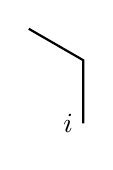
\begin{tikzpicture}[baseline=-0.2em]
      \VirutalHexagon;
      \draw [thick] (-30:0.8) node [left] {$i$} -- (30:0.8) -- (90:0.8);
    \end{tikzpicture} \, , \\
    % Loop
    \begin{tikzpicture}[baseline=-0.2em]
      \VirutalHexagon;
      \draw [very thick, draw=MaterialRed] (0,0) circle [radius=0.7];
    \end{tikzpicture}
    \enspace &= \sum_i \frac{d_i}{D} \enspace
    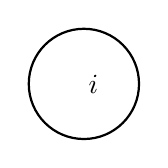
\begin{tikzpicture}[baseline=-0.2em]
      \VirutalHexagon;
      \draw [thick] (0,0) circle [radius=0.7] node [right=-0.2em] {$i$};
    \end{tikzpicture} \, .
  \end{aligned}
\end{equation}
对于邻接的六边形,我们可以在两个相邻的 $R$ 环路间执行 $F$ 移动:
\begin{align}
  \begin{tikzpicture}[baseline=-0.2em]
    \draw [thick, dotted]
      (30:1.2) -- (90:1.2) -- (150:1.2) -- (210:1.2) -- (270:1.2) -- (330:1.2)
      -- ++(-30:1.2) -- ++(30:1.2) -- ++(90:1.2) -- ++(150:1.2) -- ++(210:1.2) -- ++(270:1.2);
    \draw [very thick, draw=MaterialRed]
      (-30:0.8) -- ++(90:0.8)
      (-30:1.2) ++ (30:0.4) -- ++(90:0.8);
  \end{tikzpicture}
  \enspace &= \sum_{i,j} \biggl( \frac{d_i d_j}{D^2} \biggr)^{1/6} \enspace
  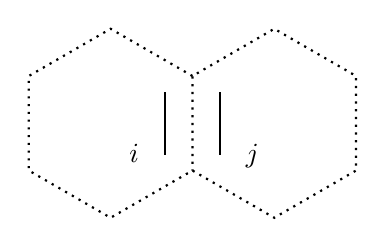
\begin{tikzpicture}[baseline=-0.2em]
    \draw [thick, dotted]
      (30:1.2) -- (90:1.2) -- (150:1.2) -- (210:1.2) -- (270:1.2) -- (330:1.2)
      -- ++(-30:1.2) -- ++(30:1.2) -- ++(90:1.2) -- ++(150:1.2) -- ++(210:1.2) -- ++(270:1.2);
    \draw [thick]
      (-30:0.8) -- ++(90:0.8)
      (-30:1.2) ++ (30:1.2-0.8) -- ++(90:0.8)
      (0.3,-0.5) node [anchor=base] {$i$}
      (1.8,-0.5) node [anchor=base] {$j$};
  \end{tikzpicture}
  \notag \\
  &= \sum_{i,j} \biggl( \frac{d_i d_j}{D^2} \biggr)^{1/6} \sum_k \sqrt{\frac{d_k}{d_i d_j}} \enspace
  \tikz [thick, baseline=-0.2em]
    \draw (90:0.6) -- +(150:1.2) node [above] {$i$} -- +(0,0) -- +(30:1.2) node [above] {$j$}
          +(0,0) -- (-90:0.6)
          +(0,0) -- +(-150:1.2) node [below] {$i$} -- +(0,0) -- +(-30:1.2) node [below] {$j$}
          (0,0) node [right] {$k$};
  \notag \\
  &= \sum_{i,j,k} \bigl( D d_i d_j \bigr)^{-1/6} d_k^{1/4} \enspace
  \begin{tikzpicture}[thick, baseline=-0.5em]
    \draw [draw=MaterialIndigo]
      (0,0) -- (270:1.2) node [below] {$k$};
    \draw [draw=MaterialPurple]
      (150:1.2) node [above=0.4, anchor=base] {$i$} -- (0,0) --
      ( 30:1.2) node [above=0.4, anchor=base] {$j$};
  \end{tikzpicture}
  \cdot \bigl( D d_i d_j \bigr)^{-1/6} d_k^{1/4} \enspace
  \begin{tikzpicture}[thick, baseline=-0.2em]
    \draw [draw=MaterialIndigo]
      (0,0) -- ( 90:1.2) node [above] {$k$};
    \draw [draw=MaterialPurple]
      (210:1.2) node [below] {$i$} -- (0,0) --
      (-30:1.2) node [below] {$j$};
  \end{tikzpicture} \, .
\end{align}
此处蓝线和紫线分别代表 $d^{-1/6}$ 和 $d^{1/4}$ 的因子。于是 $\ket{\psi_0}$ 中的每个顶点可以写成
\begin{align}
  \text{[TODO]}
\end{align}

% TODO:
在对所有的 $R$ 环路执行 $F$ 移动之后,$\ket{\psi_0}$ 现在可以表示为
\begin{equation}
  \ket{\psi_0} = ...
\end{equation}
它可以通过对位于顶点处的局域构建块进行缩并得到,并且可以用任意子基表示为
\begin{equation}
  ...
\end{equation}
这样我们就获得了六边形网格中三角形张量的对称形式:
\begin{align}
  \text{[diagram]}
  &= (d_i d_j d_k)^{-\frac14} (d_\alpha d_\beta d_\gamma)^{-\frac13} \text{[tetrahedron]} \notag \\
  &= (d_\alpha d_\beta d_\gamma)^{\frac16} (d_i d_j d_k)^{-\frac14} (d_\alpha d_\beta d_\gamma)^{-\frac12} \text{[tetrahedron]}
  \label{eq:unit-of-string-net-honeycomb}
\end{align}
对于更一般的情形,因子 $1/6$ 需要根据闭合环路中每条边的贡献进行修正。此外,我们还需要为 $B_p$ 添加额外的 $D^{-2}$ 系数,以使得 $B_p^2=B_p$。在任意三价图(每个顶点与三条边相连)中,归一化的三角形张量可以写成
\begin{equation}
  \text{[diagram]}
  = D^{-2 (1/n_\alpha + 1/n_\beta + 1/n_\gamma)}
    \bigl( d_\alpha^{1/n_\alpha} d_\beta^{1/n_\beta} d_\gamma^{1/n_\gamma} \bigr)
    (d_i d_j d_k)^{-\frac14} (d_\alpha d_\beta d_\gamma)^{-\frac12} \text{[tetrahedron]}
  \label{eq:unit-of-string-net-general}
\end{equation}
这些三角形张量每条边带有三个指标,外面的两个是\emph{虚拟指标}或\emph{辅助指标},它们会在平面内互相缩并掉;中间的一个则是\emph{物理指标},它们会伸出平面外,并且不会被缩并掉。可以看出,这实际上也是一种 PEPS 张量网络。

\begin{figure}[htb]
  \centering
  \includegraphics[width=0.6\textwidth]{images/temp/string-net-peps.pdf}
  \caption[弦网模型基态的 PEPS 张量网络表示]{弦网模型基态的 PEPS 张量网络表示。}
  \label{fig:string-net-peps}
\end{figure}

\section{奇异关联子}

\section{四面体对称性}

\section{MPO 对称性}

\section{例子}

\subsection{Fibonacci 模型}

\subsection{Ising 模型}

\chapter{Virasoro 与 Kac--Moody 代数的张量网络实现}

\section{Virasoro 与 Kac--Moody 代数简介}

\emph{共形场论} (conformal field theory, CFT) 即满足\emph{共形对称性} (conformal symmetry) 的量子场论。二维共形场论可以用很自然地用复平面上的坐标 $z$ 和 $\bar{z}$ 来描述。在共形映照 $z\to w(z)$、$\bar{z}\to\bar{w}(\bar{z})$ 下,满足
\begin{equation}
  \phi'(w,\bar{w}) = \left( \dv{w}{z} \right)^{-h} \left( \dv{\bar{w}}{\bar{z}} \right)^{-\bar{h}} \phi(z,\bar{z})
  \label{eq:quasi-primary-field}
\end{equation}
这一变换关系的场 $\phi$ 称为\emph{准初级场} (quasi-primary field),其中
\begin{equation}
  h = \frac12 \bigl( \Delta+s \bigr), \quad \bar{h} = \frac12 \bigl( \Delta-s \bigr)
\end{equation}
称为\emph{共形维数} (conformal dimension),而 $\Delta$ 和 $s$ 分别称为\emph{标度维数} (scaling dimension) 和\emph{自旋} (spin),它们确定了 $\phi$ 在标度和旋转变换下的性质。如果对任意的局部共形变换,式~\eqref{eq:quasi-primary-field} 都成立,则称 $\phi$ 为\emph{初级场} (primary field)。

根据 Noether 定理,(连续)对称性对应了守恒流。因而我们可以为局部坐标变换定义\emph{能动量张量} (energy-momentum tensor),也称\emph{应力张量} (stress tensor)。在共形对称性的条件下,能动量张量 $T^{\mu\nu}$ 可以取为对称且无迹的,即只剩下 $T(z)\coloneq T_{zz}(z)$ 和 $\bar{T}(\bar{z})\coloneq T_{\bar{z}\bar{z}}(\bar{z})$。$T$ 和 $\bar{T}$ 的共形维数分别为 $(h_T,\bar{h}_T)=(2,0)$ 和 $(h_{\bar{T}},\bar{h}_{\bar{T}})=(0,2)$,即
\begin{equation}
  \Delta_T = \Delta_{\bar{T}} = 2, \quad s_T = 2, \quad s_{\bar{T}} = -2.
\end{equation}

对于共形维数为 $(h,\bar{h})$ 初级场 $\phi$,能动量张量与它的\emph{算子积展开} (operator product expansion, OPE) 具有如下形式:
\begin{equation}
  \begin{aligned}
    T(z) \, \phi(w,\bar{z}) &\sim
      \frac{h}{(z-w)^2} \phi(w,\bar{z}) + \frac{1}{z-w} \partial_w\phi(w,\bar{z}), \\
    \bar{T}(\bar{z}) \, \phi(w,\bar{z}) &\sim
      \frac{\bar{h}}{(\bar{z}-\bar{w})^2} \phi(w,\bar{z}) + \frac{1}{\bar{z}-\bar{w}} \partial_{\bar{w}}\phi(w,\bar{z}).
  \end{aligned}
  \label{eq:t-phi-ope}
\end{equation}
而能动量张量与自身的 OPE 则可写为
\begin{equation}
  \begin{aligned}
    T(z) \, T(w) &\sim
      \frac{c/2}{(z-w)^4} + \frac{2}{(z-w)^2} T(w) + \frac{1}{z-w} \partial_w T(w), \\
    \bar{T}(\bar{z}) \, \bar{T}(\bar{w}) &\sim
        \frac{\bar{c}/2}{(\bar{z}-\bar{w})^4}
      + \frac{2}{(\bar{z}-\bar{w})^2} \bar{T}(\bar{w})
      + \frac{1}{\bar{z}-\bar{w}} \partial_{\bar{w}}\bar{T}(\bar{w}).
  \end{aligned}
\end{equation}
其中 $(c,\bar{c})$ 称为\emph{中心荷} (central charge)。

把能动量张量进行模展开,可以得到
\begin{equation}
  \begin{aligned}
    T(z)             &= \sum_{n\in\mathbb{Z}} z^{-n-2} L_n, &\quad
    L_n              &= \frac{1}{2\pi\ii} \oint z^{n+1} T(z) \, \dd z; \\
    \bar{T}(\bar{z}) &= \sum_{n\in\mathbb{Z}} \bar{z}^{-n-2} \bar{L}_n, &\quad
    \bar{L}_n        &= \frac{1}{2\pi\ii} \oint \bar{z}^{n+1} \bar{T}(\bar{z}) \, \dd\bar{z}.
  \end{aligned}
\end{equation}
式中 $L_n$ 和 $\bar{L}_n$ 称为 \emph{Virasoro 算符} (Virasoro operators),它们构成了 \emph{Virasoro 代数} (Virasoro algebra):
\begin{equation}
  \begin{aligned}
    \bigl[ L_n, L_m \bigr]
      &= (n-m) L_{n+m} + \frac{c}{12} n \bigl( n^2-1 \bigr) \delta_{n+m,0}, \\
    \bigl[ \bar{L}_n, \bar{L}_m \bigr]
      &= (n-m) \bar{L}_{n+m} + \frac{\bar{c}}{12} n \bigl( n^2-1 \bigr) \delta_{n+m,0}, \\
    \bigl[ L_n, \bar{L}_m \bigr] &= 0.
  \end{aligned}
  \label{eq:virasoro-algebra}
\end{equation}

二维共形场论可以进行\emph{径向量子化} (radial quantization),此时圆柱面可以被映射到平面上;特别地,$t\to-\infty$ 时刻会被映射到坐标原点 $z=\bar{z}=0$。因此有\emph{态—算符对应} (state-operator correspondence):
\begin{equation}
  \ket{\phi} = \lim_{z,\bar{z}\to\infty} \phi(z,\bar{z}) \ket{0},
\end{equation}
这意味着每一个场算符都可以生成一个对应的态。真空态 $\ket{0}$ 需要在全局共形变换下保持不变,这要求
\begin{equation}
  L_n \ket{0} = \bar{L}_n \ket{0} = 0, \quad n \geqslant -1.
\end{equation}
设初级场 $\phi$ 对应的态为 $\ket*{h,\bar{h}}\coloneq\phi(0,0)\ket{0}$。根据式~\eqref{eq:t-phi-ope},可知
\begin{equation}
  L_0       \ket*{h,\bar{h}} = h       \ket*{h,\bar{h}}, \quad
  \bar{L}_0 \ket*{h,\bar{h}} = \bar{h} \ket*{h,\bar{h}}, \quad
  L_n \ket*{h,\bar{h}} = \bar{L}_n \ket*{h,\bar{h}} = 0 \enspace (n > 0).
\end{equation}
利用式~\eqref{eq:virasoro-algebra} 中的对易关系,有
\begin{equation}
  \bigl[ L_0, L_{-n} \bigr] = n L_{-n}, \quad
  \bigl[ \bar{L}_0, \bar{L}_{-n} \bigr] = n \bar{L}_{-n}.
\end{equation}
可以看出 $L_{-n}\ket{0}$ 和 $\bar{L}_{-n}\ket{0}$ 分别是 $L_0$ 和 $\bar{L}_0$ 本征值为 $n$ 的本征态,因而 $L_{-n}$、$\bar{L}_{-n}$ 即可作为升算符,使得共形维数 $h$、$\bar{h}$ 增加 $n$。产生的这些态称为 $\ket*{h,\bar{h}}$ 的\emph{后代} (descendant),它们实际上也可以通过对 $\phi$ 求导得到。

\section{离散全纯性}

\section{Virasoro 与 Kac--Moody 算符的构造}

\section{能动量张量的确定}

\chapter{全息张量网络中的重整化群}


\backmatter

\bibliography{main}

\end{document}
